\documentclass[aspectratio=169]{beamer}
	\usepackage[utf8]{inputenc}		% Required for umlauts
	\usepackage[english]{babel}		% Language
	%\usepackage[sfdefault]{roboto}	% Enable sans serif font roboto
	%\usepackage{libertine}			% Enable this on Windows to allow for microtype
	\usepackage[T1]{fontenc}		% Required for output of umlauts in PDF

	\usepackage{mathtools}		% Required for formulas

	\usepackage{caption}		% Customize caption aesthetics
	\usepackage{tcolorbox}		% Fancy colored boxes
	\usepackage{xcolor}			% Highlighting
	\usepackage{soul}

	\usepackage{booktabs}		% Using pandas' LaTeX output
	\usepackage{multirow}		% Enable fancy table structure

	\usepackage{listings}		% Insert programming code
	\usepackage{graphicx}		% Required to insert images
	\usepackage{subcaption}		% Enable sub-figure
	\usepackage[space]{grffile} % Insert images baring a filename which contains spaces
	\usepackage{float}			% Allow to forcefully set the location of an object

	\usepackage[tracking=true]{microtype} % Required to change character spacing

	\usepackage[style=alphabetic,backend=biber,sorting=none,giveninits=true,isbn=false,url=false]{biblatex}
	\usepackage{csquotes}		% Ensure proper quotation of texts with babel and polyglossia with biblatex
	\usepackage{hyperref}		% Insert clickable references

	\usepackage{datetime}		% Flexible date specification
	\newcommand{\leadingzero}[1]{\ifnum#1<10 0\the#1\else\the#1\fi}
	\newcommand{\todayddmmyyyy}{\leadingzero{\day}.\leadingzero{\month}.\the\year}
	\newcommand{\mathcolorbox}[2]{\colorbox{#1}{$\displaystyle #2$}}

	\usepackage{geometry}
	\usepackage{scrextend}		% Allow arbitrary indentation

	\usepackage{color}

	\usepackage{appendixnumberbeamer}	% Fancy page numbering excluding the appendix

	% Compile notes into a separate file readable by pdfpc using a custom package which overwrite the `note` macro
	\usepackage{../pdfpcnotes}

	\makeatletter
	% Fix subfig in beamer style presentation
	\let\@@magyar@captionfix\relax

	% Insert [short title] for \section in ToC
	\patchcmd{\beamer@section}{{#2}{\the\c@page}}{{#1}{\the\c@page}}{}{}
	% Insert [short title] for \section in Navigation
	\patchcmd{\beamer@section}{{\the\c@section}{\secname}}{{\the\c@section}{#1}}{}{}
	% Insert [short title] for \subsection in ToC
	\patchcmd{\beamer@subsection}{{#2}{\the\c@page}}{{#1}{\the\c@page}}{}{}
	% Insert [short title] for \subsection in Navigation
	\patchcmd{\beamer@subsection}{{\the\c@subsection}{#2}}{{\the\c@subsection}{#1}}{}{}
	\makeatother

	\addbibresource{../literature.bib}

	\setbeamercolor{title}{fg=orange}
	\setbeamertemplate{title}{
		\color{orange}
		\textbf{\inserttitle}
	}
	\setbeamercolor{tableofcontents}{fg=orange}
	\setbeamercolor{section in toc}{fg=black}
	\setbeamercolor{subsection in toc}{fg=black}
	\setbeamertemplate{frametitle}{
		%\vspace{0.5em}
		\color{orange}
		\begin{center}
			\textbf{\insertframetitle} \\
			{\small \insertframesubtitle}
		\end{center}
	}
	\setbeamertemplate{footline}[text line]{
		\parbox{\linewidth}{
			\color{gray}
			\vspace*{-1em}
			NII 2018
			\hfill
			Gordian (\href{mailto:gordian.edenhofer@gmail.com}{gordian.edenhofer@gmail.com})
			\hfill
			\insertframenumber/\inserttotalframenumber%
		}
	}
	\setbeamertemplate{navigation symbols}{}
	\setbeamertemplate{itemize item}{\color{black}$\bullet$}
	\setbeamertemplate{itemize subitem}{\color{black}$\circ$}
	\setbeamercolor{block title}{fg=black}
	\captionsetup{font=scriptsize,labelfont={bf,scriptsize}}

	\lstset{basicstyle=\ttfamily,breaklines=true,showstringspaces=false,commentstyle=\color{red},keywordstyle=\color{blue}}

	\title{Meta-Learning~for~Recommender~Systems}
	\subtitle{``learning to learn''}
	\author[Edenhofer]{\href{mailto:gordian.edenhofer@gmail.com}{Gordian Edenhofer}}
	\institute[NII]{
		Working Group of Prof.~Dr.~Beel, Trinity College Dublin \\
		Laboratory of Prof.~Dr.~Akiko~Aizawa, Nationa Institute of Informatics
	}
	\date[Research Internship 2018]{National Institute of Informatics, \formatdate{07}{09}{2018}}
	\subject{Natural Language Processing and Machine Translation}


\begin{document}

\pagenumbering{arabic}

\begin{frame}[plain,noframenumbering]
	\titlepage%
\end{frame}

\section[Introduction]{Algorithm Selection}
\frame{\vfill\centering\tableofcontents[sectionstyle=show/shaded,subsectionstyle=show/hide]\vfill}

\subsection{Problem Definition}
\begin{frame}
	\frametitle{\insertsection}
	\framesubtitle{\insertsubsection}

	\begin{itemize}
		\item Failure to incorporate individuality of users and or items
		\begin{itemize}
			\item Collaborative filtering techniques aggregating groups of users
			\item Content-based filtering techniques measuring similarity in choice of words
		\end{itemize}
		\item One-fits-it-all approach
		\begin{itemize}
			\item Inductive bias (see~\cite{DBLP:journals/corr/abs-1708-08447})
			\note{One-fits-it-all: matrix factorization algorithm e.g.\ completely disregard descriptions and merely focuses on a rating}
			\note{One-fits-it-all: as shown by Beel et al.\ time, gender etc.\ plays a significant role}
			\item Not necessarily superior for every user and or item (see~\cite{DBLP:journals/corr/abs-1805-12118})
		\end{itemize}
	\end{itemize}
\end{frame}

\subsection{Proposal}
\begin{frame}
	\frametitle{\insertsection}
	\framesubtitle{\insertsubsection}

	\begin{itemize}
		\item Stacked ensemble learning
		\begin{itemize}
			\item Usually only incorporate a small subset of algorithm classes (cf.\ Random Forest)
			\item Computational performance penalty of complex approaches
		\end{itemize}
		{
			\setbeamertemplate{itemize item}{\color{black}$\Rightarrow$}
			\item Algorithm selection as machine learning task: \colorbox{yellow}{\bf{switching hybrid ensemble}}
		}
		\begin{itemize}
			\item Best algorithm for given user and or item
			\item Minimal computational overhead (compared to stacked ensemble models)
		\end{itemize}
		\note{Switching hybrid ensemble: `switching' as it changes underlying algorithm used for predictions}
		\note{Switching hybrid ensemble: `hybrid' as it utilizes multiple multitude of filtering techniques}
		\note{Switching hybrid ensemble: `ensemble' as it processes results based on a collection of algorithms}
	\end{itemize}
\end{frame}

\section[Literature]{Meta-Learning}
\frame{\vfill\centering\tableofcontents[sectionstyle=show/shaded,subsectionstyle=show/hide]\vfill}

\subsection{Abstract Concept}
\begin{frame}
	\frametitle{\insertsection}
	\framesubtitle{\insertsubsection}

	\begin{itemize}
		\item Machine learning on metadata -- ``learning to learn''
		\item Learning subsystem
		\item Meta-learner on top of learning subsystem (cf.\ stacked ensemble)
		\begin{itemize}
			\item Pre-processed meta-features, e.g.~corpus statistics
			\item Subsystem runtime information and or its estimate as new input
		\end{itemize}
	\end{itemize}
\end{frame}

\subsection{Related Work}
\begin{frame}
	\frametitle{\insertsection}
	\framesubtitle{\insertsubsection}

	\begin{itemize}
		\item `One-at-a-time'~\cite{DBLP:journals/corr/abs-1805-12118}
		\begin{itemize}
			\item Main inspiration for this research
			\item Outline of the concepts and exploration of initial approaches
		\end{itemize}
		\note{One-at-a-time: micro- and macro- recommenders}
		\note{One-at-a-time: theoretical best}
		\note{One-at-a-time: failure to achieve good results using simple regression}
		\item `Metalearning and Recommender Systems'~\cite{CUNHA2018128}
		\note{ML and RecSys: recommender systems evaluationg and accuracy measures}
		\note{ML and RecSys: overview of recommender systems: Collaborative filtering, content-based filtering, social-based filtering, knowledge-based filtering, hybrid filtering, context-aware filtering, deep learning-based recommendations and group recommendations}
		\note{ML and RecSys: recommender systems evaluationg and accuracy measures}
		\note{ML and RecSys: meta-features, Meta-targets, Meta-level}
		\item `When Recommenders Fail'~\cite{Ekstrand:2012:RFP:2365952.2366002}
		\note{When Recommendations Fail: missing user and item feature in MovieLense data for proper algorithm selection}
	\end{itemize}
\end{frame}

\section[Methodology]{Meta-Learning System Design}
\frame{\vfill\centering\tableofcontents[sectionstyle=show/shaded,subsectionstyle=show/hide]\vfill}

\subsection{Learning Subsystem}
\begin{frame}
	\frametitle{\insertsection}
	\framesubtitle{\insertsubsection}

	\begin{itemize}
		\item Cross-validation using $5$ folds
		\item Top-N accuracy using the recall
		\begin{itemize}
			\item Randomized subset of $100$ projects the user has not donated to
			\item One project to which the user has donated to
			\item Recall@N is predicted position of donated project in the subset of $101$ projects
		\end{itemize}
	\end{itemize}

	\begin{table}
		\scriptsize
		\centering
		\begin{tabular}{l|lll}
			Filtering method & Algorithm & Computational method & Yields \\
			\hline
			\hline
			collaborative & KNN & neirest-neighbor (2-norm) & RMSE, MAE, \colorbox{yellow}{Recall@N} \\
			& SVD & matrix factorization & RMSE, MAE, \colorbox{yellow}{Recall@N} \\
			\hline
			content-based & TF-IDF & term frequency & cosine similarity, \colorbox{yellow}{Recall@N} \\
			\hline
			content-based, neural network & fastText & word-embedding & cosine similarity, \colorbox{yellow}{Recall@N} \\
		\end{tabular}
		\caption{Architecture of the learning subsystem with a list of properties for each algorithm.}
	\end{table}
\end{frame}

\subsection{Meta-Learner}
\begin{frame}
	\frametitle{\insertsection}
	\framesubtitle{\insertsubsection}

	\begin{itemize}
		\item Holdout-validation using $80\%$ train-test-split
		\item Meta-features
		\begin{itemize}
			\item User-, item- and transaction-information
			\note{User information: location, teacher-status}
			\note{Item information: location, metro-type, category, lunch-subsidies}
			\note{Transaction information: time}
			\item Corpus statistics
			\note{Corpus statistics: value counts for user and item}
			\note{Corpus statistics: looking into adding much more meta-features}
		\end{itemize}
		\item Meta-learner approaches
		\begin{itemize}
			\item Error prediction
			\item Transaction classification
		\end{itemize}
	\end{itemize}
\end{frame}

\begin{frame}
	\frametitle{\insertsection}
	\framesubtitle{\insertsubsection}

	\begin{figure}
		\centering
		\subcaptionbox{Error prediction}{
			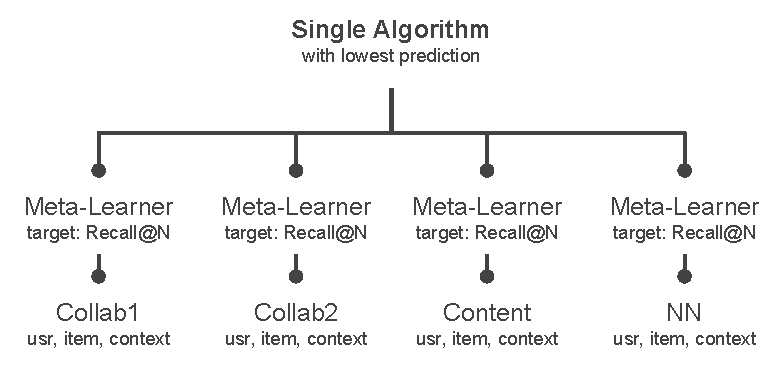
\includegraphics[width=0.45\textwidth,height=\textheight,keepaspectratio]{{{../res/Meta-Learner Architecture: Error prediction algorithm}}}
			}
		\subcaptionbox{Classification}{
			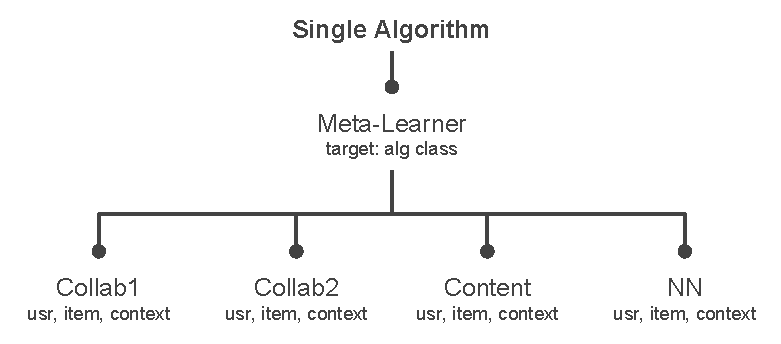
\includegraphics[width=0.45\textwidth,height=\textheight,keepaspectratio]{{{../res/Meta-Learner Architecture: Classification algorithm}}}
		}
		\caption{Meta-learner architecture for an error predicting and a classification approach.}
	\end{figure}
	\note{Error predicting approach: Separate meta-learner predicting the Recall@N for each algorithm in the subsystem}
	\note{Error predicting approach: Accuracy is measured using the algorithm with lowest predicted Recall@N}
	\note{Classification approach: Transaction is assigned to the class of the algorithm with the lowest Recall@N}
	\note{Classification approach: Meta-learner predicts class of the transaction}
	\note{Classification approach: Accuracy is measured using the algorithm of the predicted class}
\end{frame}

\section[Results]{Meta-Learning Experiment}
\frame{\vfill\centering\tableofcontents[sectionstyle=show/shaded,subsectionstyle=show/hide]\vfill}

\subsection{Learning Subsystem}
\begin{frame}
	\frametitle{\insertsection}
	\framesubtitle{\insertsubsection}

	\begin{figure}
		\centering
		\includegraphics[width=\textwidth,height=0.6\textheight,keepaspectratio]{{{../res/Learning subsystem - Distribution of position in Top-N test set for various algorithms}}}
		\caption{Distribution of the positon of the project to which the user donated to in a set of $100$ projects the user has not donated to. Results are shown for a subset of the learning subsystem.}
	\end{figure}
\end{frame}

\begin{frame}
	\frametitle{\insertsection}
	\framesubtitle{\insertsubsection}

	\begin{figure}
		\centering
		\includegraphics[width=\textwidth,height=0.6\textheight,keepaspectratio]{{{../res/Learning subsystem - Position in Top-N test set for various algorithms}}}
		\caption{Statistical features of the distribution of the donated item position in the Recall@N test set. Hereby, the orange line is indicating the median, the green line the mean.}
	\end{figure}
\end{frame}

\subsection{Meta-Learner}
\begin{frame}
	\frametitle{\insertsection}
	\framesubtitle{\insertsubsection}

	\scalebox{.47}{
		\centering
		% Extract the table via the following command and add the necessary midrule to separate inputs from targets
		% meta_items.loc[train_idx][sorted(feature_columns) + ['SubalgorithmCategory'] + sorted(alg_acc_to_alg_columns.keys())].head(5).transpose().to_latex('meta_items: table head.tex', multirow=True, header=False)
		\input{"../res/meta_items: table head"}
	}
\end{frame}

\begin{frame}
	\frametitle{\insertsection}
	\framesubtitle{\insertsubsection}

	\begin{figure}
		\centering
		\includegraphics[width=\textwidth,height=0.6\textheight,keepaspectratio]{{{../res/Meta-learner as Classifier and Error Predictor - Average position in Top-N test set for various meta-learner algorithms}}}
		\caption{Performance of various meta-learners in comparison to the overall best algorithm. Meta-learners are used as classifiers (CL) as well as for error predictions (EP).}
	\end{figure}
\end{frame}

\section{Outlook}
\frame{\vfill\centering\tableofcontents[sectionstyle=show/shaded,subsectionstyle=show/hide]\vfill}

\subsection{Further Meta-Features \& Collaborative Filters}
\begin{frame}
	\frametitle{\insertsection}
	\framesubtitle{\insertsubsection}

	\begin{itemize}
		\item Novel meta-features
		\begin{itemize}
			\item Statistical features of the dataset
			\item Pre-calculated values of combined of meta-features
		\end{itemize}
		\item Explore further collaborative filtering techniques
		\begin{itemize}
			\item Filtering based on common user features, e.g.~location
			\item Possibly implement novel and previously unexplored algorithms (?)
		\end{itemize}
		\item Alternative datasets
	\end{itemize}
\end{frame}

\section*{Summary}
\subsection{\inserttitle}

\begin{frame}
	\frametitle{\insertsection}
	\framesubtitle{\insertsubsection}

	\begin{itemize}
		\note{Corpus selection: DonorsChoose.org dataset features user, item and context information}
		\item Learning subsystem
		\begin{itemize}
			\item Collaborative filtering techniques, i.e.~KNN and SVD
			\item Content-based filtering technique, i.e.~TF-IDF
			\item Content-based neural network approach, i.e.~word-embedding using fastText
		\end{itemize}
		\item Meta-feature sanitization
		\item Algorithm selection via meta-learner systems
		\begin{itemize}
			\item Error prediction
			\item Classification
		\end{itemize}
	\end{itemize}
\end{frame}

\appendix

\begin{frame}[shrink=20]
	\frametitle{Bibliography}

	\printbibliography%
\end{frame}

\end{document}
